% Options for packages loaded elsewhere
\PassOptionsToPackage{unicode,linktoc=all}{hyperref}
\PassOptionsToPackage{hyphens}{url}
\PassOptionsToPackage{dvipsnames,svgnames,x11names}{xcolor}
%
\documentclass[
  a4paper,
]{article}
\usepackage{amsmath,amssymb}
\usepackage{lmodern}
\usepackage{iftex}
\ifPDFTeX
  \usepackage[T1]{fontenc}
  \usepackage[utf8]{inputenc}
  \usepackage{textcomp} % provide euro and other symbols
\else % if luatex or xetex
  \usepackage{unicode-math}
  \defaultfontfeatures{Scale=MatchLowercase}
  \defaultfontfeatures[\rmfamily]{Ligatures=TeX,Scale=1}
\fi
% Use upquote if available, for straight quotes in verbatim environments
\IfFileExists{upquote.sty}{\usepackage{upquote}}{}
\IfFileExists{microtype.sty}{% use microtype if available
  \usepackage[]{microtype}
  \UseMicrotypeSet[protrusion]{basicmath} % disable protrusion for tt fonts
}{}
\makeatletter
\@ifundefined{KOMAClassName}{% if non-KOMA class
  \IfFileExists{parskip.sty}{%
    \usepackage{parskip}
  }{% else
    \setlength{\parindent}{0pt}
    \setlength{\parskip}{6pt plus 2pt minus 1pt}}
}{% if KOMA class
  \KOMAoptions{parskip=half}}
\makeatother
\usepackage{xcolor}
\IfFileExists{xurl.sty}{\usepackage{xurl}}{} % add URL line breaks if available
\IfFileExists{bookmark.sty}{\usepackage{bookmark}}{\usepackage{hyperref}}
\hypersetup{
  pdftitle={Solving a Mathematics Olympiad problem},
  pdfauthor={R (Chandra) Chandrasekhar},
  pdflang={en-GB},
  colorlinks=true,
  linkcolor={DarkOliveGreen},
  filecolor={Purple},
  citecolor={DarkKhaki},
  urlcolor={Maroon},
  pdfcreator={LaTeX via pandoc}}
\urlstyle{same} % disable monospaced font for URLs
\usepackage[margin=25mm]{geometry}
\usepackage{longtable,booktabs,array}
\usepackage{calc} % for calculating minipage widths
% Correct order of tables after \paragraph or \subparagraph
\usepackage{etoolbox}
\makeatletter
\patchcmd\longtable{\par}{\if@noskipsec\mbox{}\fi\par}{}{}
\makeatother
% Allow footnotes in longtable head/foot
\IfFileExists{footnotehyper.sty}{\usepackage{footnotehyper}}{\usepackage{footnote}}
\makesavenoteenv{longtable}
\usepackage{graphicx}
\makeatletter
\def\maxwidth{\ifdim\Gin@nat@width>\linewidth\linewidth\else\Gin@nat@width\fi}
\def\maxheight{\ifdim\Gin@nat@height>\textheight\textheight\else\Gin@nat@height\fi}
\makeatother
% Scale images if necessary, so that they will not overflow the page
% margins by default, and it is still possible to overwrite the defaults
% using explicit options in \includegraphics[width, height, ...]{}
\setkeys{Gin}{width=\maxwidth,height=\maxheight,keepaspectratio}
% Set default figure placement to htbp
\makeatletter
\def\fps@figure{htbp}
\makeatother
\setlength{\emergencystretch}{3em} % prevent overfull lines
\providecommand{\tightlist}{%
  \setlength{\itemsep}{0pt}\setlength{\parskip}{0pt}}
\setcounter{secnumdepth}{-\maxdimen} % remove section numbering
\newlength{\cslhangindent}
\setlength{\cslhangindent}{1.5em}
\newlength{\csllabelwidth}
\setlength{\csllabelwidth}{3em}
\newlength{\cslentryspacingunit} % times entry-spacing
\setlength{\cslentryspacingunit}{\parskip}
\newenvironment{CSLReferences}[2] % #1 hanging-ident, #2 entry spacing
 {% don't indent paragraphs
  \setlength{\parindent}{0pt}
  % turn on hanging indent if param 1 is 1
  \ifodd #1
  \let\oldpar\par
  \def\par{\hangindent=\cslhangindent\oldpar}
  \fi
  % set entry spacing
  \setlength{\parskip}{#2\cslentryspacingunit}
 }%
 {}
\usepackage{calc}
\newcommand{\CSLBlock}[1]{#1\hfill\break}
\newcommand{\CSLLeftMargin}[1]{\parbox[t]{\csllabelwidth}{#1}}
\newcommand{\CSLRightInline}[1]{\parbox[t]{\linewidth - \csllabelwidth}{#1}\break}
\newcommand{\CSLIndent}[1]{\hspace{\cslhangindent}#1}
\ifLuaTeX
\usepackage[bidi=basic]{babel}
\else
\usepackage[bidi=default]{babel}
\fi
\babelprovide[main,import]{british}
% get rid of language-specific shorthands (see #6817):
\let\LanguageShortHands\languageshorthands
\def\languageshorthands#1{}
% $HOME/.pandoc/defaults/latex-header-includes.tex
% Common header includes for both lualatex and xelatex engines.
%
% Preliminaries
%
% \PassOptionsToPackage{rgb,dvipsnames,svgnames}{xcolor}
% \PassOptionsToPackage{main=british}{babel}
\AtBeginEnvironment{quote}{\small}
\AtBeginEnvironment{quotation}{\small}
\AtBeginEnvironment{longtable}{\centering}
%
% Packages that are useful to include
%
\usepackage{graphicx}
\usepackage{subcaption}
\usepackage[inkscapeversion=1]{svg}
\usepackage[defaultlines=4,all]{nowidow}
\usepackage[capitalize,noabbrev]{cleveref}
\usepackage{etoolbox}
\usepackage{fontsize}
\usepackage{newunicodechar}
\usepackage{pdflscape}
\usepackage{fnpct}
\usepackage{parskip}
  \setlength{\parindent}{0pt}
\usepackage[style=american]{csquotes}
% \usepackage{setspace} Use the <fontname-plus.tex> files for setspace
%
\usepackage{esdiff} % for derivative symbols
\usepackage{amsmath}
% noto-plus.tex
% Font-setting header file for use with Pandoc Markdown
% to generate PDF via LuaLaTeX.
% The main font is Noto Serif.
% Other main fonts are also available in appropriately named file.
\usepackage{fontspec}
\usepackage{setspace}
\setstretch{1.3}
%
\defaultfontfeatures{Ligatures=TeX,Scale=MatchLowercase,Renderer=Node} % at the start always
%
% For English
% See also https://tex.stackexchange.com/questions/574047/lualatex-amsthm-polyglossia-charissil-error
% We use Node as Renderer for the Latin Font and Greek Font and HarfBuzz as renderer ofr Indic fonts.
%
\babelfont{rm}[Script=Latin,Scale=1]{NotoSerif}% Config is at $HOME/texmf/tex/latex/NotoSerif.fontspec
%
\babelfont{sf}[Script=Latin]{SourceSansPro}% Config is at $HOME/texmf/tex/latex/SourceSansPro.fontspec
%
\babelfont{tt}[Script=Latin]{FiraMono}% Config is at $HOME/texmf/tex/latex/FiraMono.fontspec
%
% Sanskrit, Tamil, and Greek fonts
%
\babelprovide[import, onchar=ids fonts]{sanskrit}
\babelprovide[import, onchar=ids fonts]{tamil}
\babelprovide[import, onchar=ids fonts]{greek}
%
\babelfont[sanskrit]{rm}[Scale=1.1,Renderer=HarfBuzz,Script=Devanagari]{NotoSerifDevanagari}
\babelfont[sanskrit]{sf}[Scale=1.1,Renderer=HarfBuzz,Script=Devanagari]{NotoSansDevanagari}
\babelfont[tamil]{rm}[Renderer=HarfBuzz,Script=Tamil]{NotoSerifTamil}
\babelfont[tamil]{sf}[Renderer=HarfBuzz,Script=Tamil]{NotoSansTamil}
\babelfont[greek]{rm}[Script=Greek]{GentiumBookPlus}
%
% Math font
%
\usepackage{unicode-math} % seems not to hurt % fallabck
\setmathfont[bold-style=TeX]{STIX Two Math}
%
%
% Other fonts
%
\newfontfamily{\emojifont}{Symbola}
%

\usepackage{titling}
\usepackage{fancyhdr}
    \pagestyle{fancy}
    \fancyhead{}
    \fancyfoot{}
    \renewcommand{\headrulewidth}{0.2pt}
    \renewcommand{\footrulewidth}{0.2pt}
    \fancyhead[LO,RE]{\scshape\thetitle}
    \fancyfoot[CO,CE]{\footnotesize Copyright © 2006\textendash\the\year, R (Chandra) Chandrasekhar}
    \fancyfoot[RE,RO]{\thepage}
\newfontfamily{\regulariconfont}{Font Awesome 6 Free Regular}[Color=Grey]
\newfontfamily{\solidiconfont}{Font Awesome 6 Free Solid}[Color=Grey]
\newfontfamily{\brandsiconfont}{Font Awesome 6 Brands}[Color=Grey]
%
% Direct input of Unicode code points
%
\newcommand{\faEnvelope}{\regulariconfont\ ^^^^f0e0\normalfont}
\newcommand{\faMobile}{\solidiconfont\ ^^^^f3cd\normalfont}
\newcommand{\faLinkedin}{\brandsiconfont\ ^^^^f0e1\normalfont}
\newcommand{\faGithub}{\brandsiconfont\ ^^^^f09b\normalfont}
\newcommand{\faAtom}{\solidiconfont\ ^^^^f5d2\normalfont}
\newcommand{\faPaperPlaneRegular}{\regulariconfont\ ^^^^f1d8\normalfont}
\newcommand{\faPaperPlaneSolid}{\solidiconfont\ ^^^^f1d8\normalfont}

%
% The block below is commented out because of Tofu glyphs in HTML
%
% \newcommand{\faEnvelope}{\regulariconfont\ \normalfont}
% \newcommand{\faMobile}{\solidiconfont\ \normalfont}
% \newcommand{\faLinkedin}{\brandsiconfont\ \normalfont}
% \newcommand{\faGithub}{\brandsiconfont\ \normalfont}
\ifLuaTeX
  \usepackage{selnolig}  % disable illegal ligatures
\fi

\title{Solving a Mathematics Olympiad problem}
\author{R (Chandra) Chandrasekhar}
\date{2023-03-15 | 2023-03-19}

\begin{document}
\maketitle

\thispagestyle{empty}


\hypertarget{a-problem-that-beckoned}{%
\subsection{A problem that beckoned}\label{a-problem-that-beckoned}}

During a casual tour of the Web, my attention was drawn to a problem
that was stated so simply that it beckoned an attempt at a solution. It
was purported to be from a
\href{https://www.imo-official.org/}{Mathematical Olympiad}, which
raised its attractiveness index, as such problems are known to
strenuously exercise the grey cells, while still retaining the charm of
a sport. Only later did I find out that the problem I had written down
had omitted an important constraint that made the problem all the more
memorable. This is an account of my escapade into the land of
mathematics in search of a solution to an intriguing problem.

\hypertarget{the-problem}{%
\subsection{The problem}\label{the-problem}}

The problem, as I first came across it, was posed thus.
\begin{equation}\protect\hypertarget{eq:problem}{}{
\text{If}\quad
x + xy + y = 54
}\label{eq:problem}\end{equation} what is \(x + y\)?

If you are good at mathematics, or relish a challenge, do not read
further until you have given this problem your very best shot. After
that, do read on.

\hypertarget{first-thoughts}{%
\subsection{First thoughts}\label{first-thoughts}}

At first, I thought that this problem was too easy to be featured in a
Mathematics Olympiad\footnote{I have not checked the if, the which, the
  when, and the level of the Olympiad, but simply took on the problem in
  good faith.}. After all, the problem statement would be intelligible
to anyone who has gone through mathematics up to middle (or secondary)
school level. But after a short while, I realized that it posed some
definite challenges.

In this blog, I am not setting out to expound a blazingly fast method of
solution, nor am I attempting mathematical terseness. I will be
discursive because I want to \emph{savour} the problem in all its
aspects, as they suggested themselves to me. I also hope that, by so
doing, I stimulate mathematical thinking in my readers, and give them an
experience of the mathematical adventure, if nothing else.

\hypertarget{a-pictorial-approach}{%
\subsection{A pictorial approach}\label{a-pictorial-approach}}

Mathematics may be approached through pictures, or through words, or
through a combination of both. Here, I am going to try pictures first.
This means graphing the curve defined by \cref{eq:problem} and wresting
as many insights as possible from that representation.

How do we graph the given curve? And after that, how do we obtain the
value of \(x + y\), which is our ultimate goal? Let us see how this
approach pans out.

For a start, I am \href{https://www.thefreedictionary.com/loath}{loath}
to graph curves by hand. So, I went to my favourite graphing destination
on the Web, \href{https://www.desmos.com}{Desmos}, to experiment with
the given curve. The \href{https://www.desmos.com/calculator}{Desmos
Graphing Calculator} offers the easiest and laziest route to visualize
algebraic curves.

I typed in
\href{https://www.desmos.com/calculator/nwkikstcm6}{\(x + xy + y = 54\)}
into the textbox for the first graph and got what seemed at first sight
to be a pair of curves for a rectangular hyperbola of the form
\(xy = k\) where \(k\) is some constant (or number).

\begin{figure}
\hypertarget{fig:one}{%
\centering
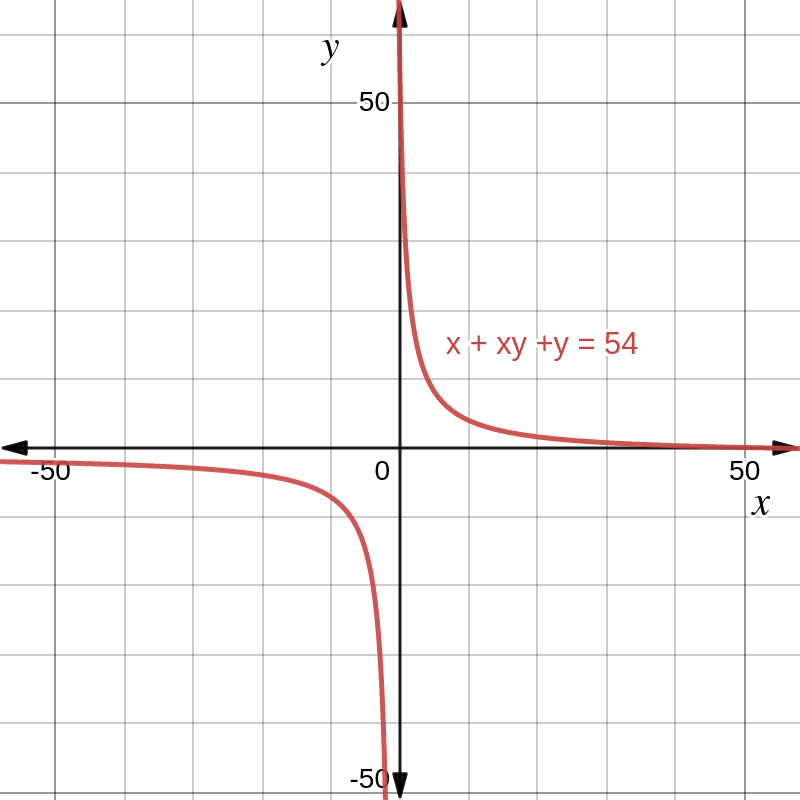
\includegraphics[width=0.75\textwidth,height=\textheight]{images/olympiad-one.png}
\caption{A graph of the curve \(x + xy + y = 54\).}\label{fig:one}
}
\end{figure}

From \cref{fig:one}, we can deduce the following:

\begin{enumerate}
\def\labelenumi{(\alph{enumi})}
\item
  The curve \emph{looks like} a rectangular hyperbola, with its two
  portions lying \emph{largely} in the first and third quadrants.
\item
  If we re-write \cref{eq:problem} to have only \(y\) on the left hand
  side (LHS), we get:
  \begin{equation}\protect\hypertarget{eq:hyperbola}{}{
  y = \frac{54-x}{x+1} = \frac{54}{x+1} -\frac{x}{x+1} \approx \frac{54}{x} - 1 \approx -1 \; \mbox{for large $x$}
  }\label{eq:hyperbola}\end{equation} Wonder no more why the curve
  resembles a rectangular hyperbola. Its horizontal (and vertical)
  \href{https://en.wikipedia.org/wiki/Asymptote}{asymptotes} equal
  \(-1\). That is why it lies \emph{largely} in the first and third
  quadrants.
\item
  Only those points \((x, y)\) that satisfy \cref{eq:problem} are
  relevant for our second condition \(x + y\), i.e., our solution space
  is defined by the curves comprising the two halves of the plotted
  graph. The rest of the \(xy\) plane does not contain the solution we
  seek.
\item
  Since we are after the value of \(x + y\), we can plot the
  \emph{family of curves} \(x + y = k\) where \(k\) is some real
  constant. This is done in \cref{fig:two}. The two straight lines that
  are tangent can be derived from calculation, as shown in the
  \protect\hyperlink{appendix}{Appendix} at the end. They represent
  limiting cases of the values of \(k\) within which a solution
  \emph{cannot} lie.
\end{enumerate}

\begin{figure}
\hypertarget{fig:two}{%
\centering
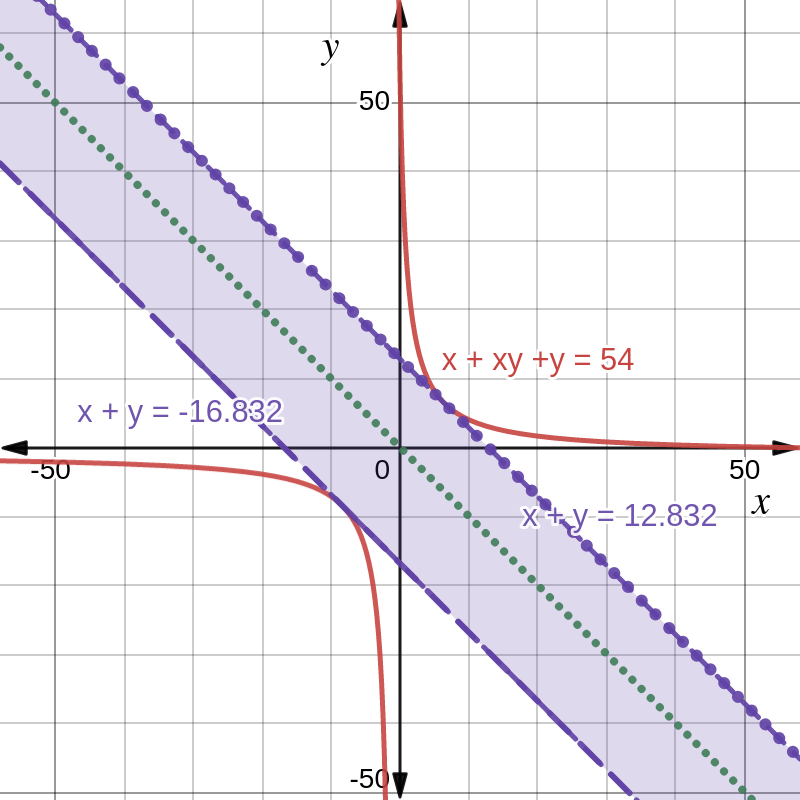
\includegraphics[width=0.75\textwidth,height=\textheight]{images/olympiad-two.png}
\caption{The \emph{family of curves} \(x + y = k\) is plotted for three
values of \(k\). The green dotted line represents \(x + y = 0\). The two
purple lines represent \(x + y = 12.832\) and \(x + y = -16.832\). The
solution \emph{cannot} lie within the purple region, bounded by the
latter two lines because no intersection with the nonlinear red curve is
possible there. The purple lines are shown broken because the purple
region does not include these two lines themselves.}\label{fig:two}
}
\end{figure}

To look for possible solutions, we need to plot straight lines like
\(x + y = 20\) and \(x + y = -30\) which will intersect the red curves
as shown in \cref{fig:three}.

\begin{figure}
\hypertarget{fig:three}{%
\centering
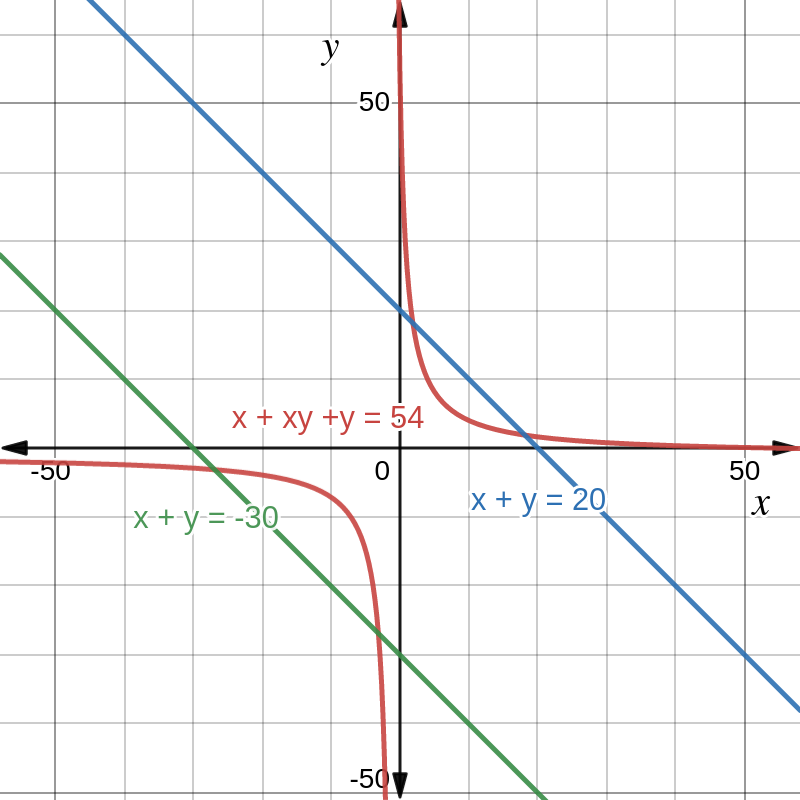
\includegraphics[width=0.75\textwidth,height=\textheight]{images/olympiad-three.png}
\caption{Two straight lines that intersect the curve
\(x + xy + y = 54\). The respective solutions are \(x + y = 20\) and
\(x + y = -30\).}\label{fig:three}
}
\end{figure}

It should be clear that there is nothing special about the numbers
\(20\) or \(-30\). So, there is an infinity of possible solutions for
\(x + y = k\) in two disjoint sets: \(x + y \geq 12.832\) and
\(x + y \leq -16.832\), as shown in the
\protect\hyperlink{appendix}{Appendix}.

Although we have reached the end of the prescribed quest, there is a
sense of hollowness, because there is no \emph{unique} solution (set),
except that the solution can lie anywhere along the red curves, and is
forbidden in the purple region of \cref{fig:two}.

It is appropriate now to take a breather and re-examine all assumptions.
Perhaps, it is the time to ruminate philosophically about mathematical
problems.

\hypertarget{mathematics-problems-and-detective-novels}{%
\subsection{Mathematics problems and detective
novels}\label{mathematics-problems-and-detective-novels}}

Mathematics problems function like detective novels. The author of a
detective novel enters into an implicit understanding with the reader,
that the clues will be peppered throughout the novel, which when viewed
as a whole, will lead to a \emph{single} culprit, preferably at the end
of the novel. If there were still ten possible culprits at the end of
the novel, the author would have completely let down the reader's
expectations, and cheated him or her of the reward of discovery for the
time spent reading the novel.

A similar compact holds between the one who poses a mathematics problem
and the student who is expected to solve it. If a problem has no
solutions, or has countless solutions, it will not necessarily enthrall
the student, especially at school level. Indeed, it will be considered a
breach of faith if either of these two conditions held.

It is unlikely that an Olympiad problem in mathematics will indulge in
such antics. What was the \emph{exact wording} of the problem?

\hypertarget{the-all-important-constraint}{%
\subsection{The all-important
constraint}\label{the-all-important-constraint}}

A more careful sweep of the Web unearthed a more precise statement of
the problem, which included a constraint. For completeness, the problem
is re-stated here:

If \(x\) and \(y\) are \emph{both positive integers}, and \[
x + xy + y = 54
\] what is \(x + y\)?

By restricting the numbers to be positive, we may discard the entire
solution set in the fourth quadrant, as well as any solutions that
intersect near the (negative-valued) asymptotes. Moreover, by
restricting the solution to integers, we are changing the domain of the
solution from a quadrant of the real plane to a
\href{https://mathworld.wolfram.com/PointLattice.html}{\emph{point
lattice}} in the first quadrant. The solution set has thus changed from
\href{https://mathworld.wolfram.com/UncountablyInfinite.html}{uncountably
infinite} to
\href{https://mathworld.wolfram.com/CountablyInfinite.html}{countably
infinite}.

If you observe \cref{fig:three} carefully, when \(k\) is large and
positive, the intersection with the given curve will occur near the
values of the asymptotes. One way to identify the solution is to vary
\(k\) in the straight line \(x + y = k\) by animation, and to identify
cases where the intersection occurs at \emph{integer values} of \(x\)
and \(y\). If you are curious how that will look like, go to
\href{https://www.desmos.com/calculator/1mklcrdbxw}{this animation at
the Desmos website} to see what happens to the solution as \(k\) varies
between \(-30\) and \(30\).

But trying to identify a solution for integers \(x\) and \(y\), by
pausing the animation every so often, and looking for whole numbers as
the co-ordinates of intersection, will be like yanking a piece of
luggage from a fast-moving carousel in an airport. It will be a hit or
miss operation rather than a dignified mathematical solution. So, let us
switch from the pictorial to the verbal. Let algebra bring to bear its
considerable prowess on this problem.

\hypertarget{algebra-to-the-rescue}{%
\subsection{Algebra to the rescue}\label{algebra-to-the-rescue}}

Let us shuffle the components of \cref{eq:problem} in an effort to
introduce even more symmetry, and gain a deeper insight:
\begin{equation}\protect\hypertarget{eq:three}{}{
\begin{aligned}
x + xy + y &= 54\\
x(1 + y) + y &= 54\; ; \mbox{add one to each side} \\
x(1 + y) + y + 1 &= 55\\
x(y + 1) + (y + 1) &= 55\\
(y + 1)(x + 1) &= 55\\
\end{aligned}
}\label{eq:three}\end{equation}

\hypertarget{why-products-over-sums}{%
\subsubsection{Why products over sums?}\label{why-products-over-sums}}

Take a look at \cref{eq:three}. Given that we are asked to evaluate
\(x + y\), why did we try to express the number 55 as a \emph{product}
of two numbers on the LHS, rather than as the \emph{sum} of two numbers?

Decomposing a number \(n\) into a sum of numbers is called
\href{https://mathworld.wolfram.com/Partition.html}{\emph{additive
partitioning}}, and is represented by the function \(p(n)\), while
decomposing a number into a product of numbers is called
\href{https://mathworld.wolfram.com/UnorderedFactorization.html}{\emph{multiplicative
partitioning} or \emph{unordered factorization}} and is represented by
the expression \(f(n)\) {[}\protect\hyperlink{ref-brown-2017}{1}{]}.

Consider the number \(6\). We may express it as a sum, using the numbers
from \(1\) to \(6\), in eleven different ways, i.e., \(p(6) = 11\). But
we may express it in only two different ways as a product, i.e.,
\(f(n)=2\). Note that we we are talking of \emph{distinct}
decompositions.

It is tempting to speculate that for any positive integer \(n\),
\(p(n) \geq f(n)\), but I have not seen any proof of this statement. For
our purposes though, it is patently reasonable\footnote{Surprisingly,
  research into the multiplicative partition of a positive integer seems
  to be a relatively recent endeavour
  {[}\protect\hyperlink{ref-dodd-1987}{2}{]}. So, I am hand-waving here.}
to claim that the number of ways in which the number \(55\) may be
decomposed as a product is far fewer than the number of ways in which it
can be decomposed as a sum, i.e., \(f(n) < p(n)\). And that is why we
sought to write the LHS of the last line of \cref{eq:three} as a product
rather than as a sum.

\hypertarget{multiplicative-partitions-of-55}{%
\subsubsection{\texorpdfstring{Multiplicative partitions of
\(55\)}{Multiplicative partitions of 55}}\label{multiplicative-partitions-of-55}}

The number 55 may be decomposed into these four \emph{unique}
factors---meaning that order does not matter: \(1, 5, 11,\) and
\(55\)\footnote{It should be blindingly obvious that
  \(1 \times 55 = 55\) and that \(5 \times 11 = 55\)
  \emojifont{😉}\normalfont}. The fact that \(5\) and \(11\) are
\href{https://mathworld.wolfram.com/PrimeFactor.html}{prime numbers} and
that their product is \(55\) has helped whittle down the number of
factors.

Let us examine the possible solutions, one by one. If we assign the
number \(1\) to \(x + 1\), then \(x\) must be zero. But we have been
told that \(x\) and \(y\) are both positive integers, meaning that they
cannot be zero or negative. \emph{So, the factor-pair \(1\) and \(55\)
is not valid}.

We may now write \cref{eq:three} as:
\begin{equation}\protect\hypertarget{eq:solution}{}{
(x+1)(y+1) = 55 = 5\times 11
}\label{eq:solution}\end{equation} If we set \(x + 1 = 5\), we get
\(x = 4\). Likewise, setting \(y + 1 = 11\) gives \(y = 10\). Therefore,
\(x + y = 4 + 10 = 14\). It should be abundantly clear that \(x\) and
\(y\) could interchange their values but their sum will still be the
same. So, the solution to the problem is \(x + y = 14\), and we are home
and dry.

\hypertarget{the-final-picture}{%
\subsubsection{The final picture}\label{the-final-picture}}

To get a sense of finality, let us see the graphical representation of
our algebraic result in \cref{fig:four} below.

\begin{figure}
\hypertarget{fig:four}{%
\centering
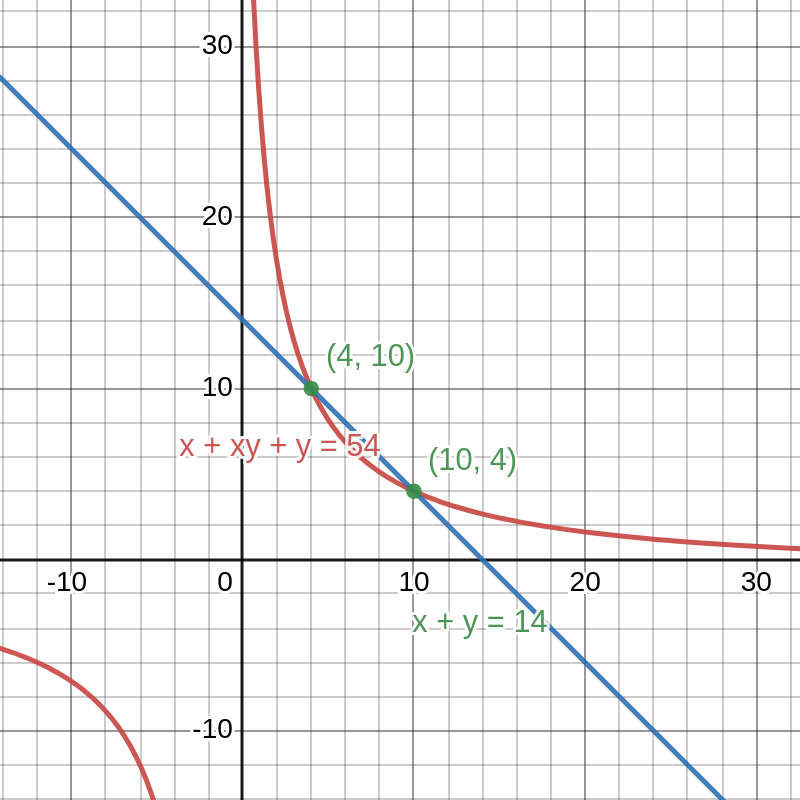
\includegraphics[width=0.75\textwidth,height=\textheight]{images/olympiad-four.png}
\caption{The line \(x + y = 14\) intersects the curve \(x + xy +y = 54\)
at \emph{two} points: \((10, 4)\) and \((4, 10)\). Thus although
\(x + y = 14\) is a \emph{single} line---and the required solution---if
we had been asked for the points of intersection, we would have to
enumerate \emph{both} points.}\label{fig:four}
}
\end{figure}

\hypertarget{appendix}{%
\subsection{Appendix}\label{appendix}}

The somewhat magic numbers \(12.832\) and \(-16.832\) in \cref{fig:two}
were not drawn out of thin air, but are the result of simple
calculations. It should be clear that the straight lines in
\cref{fig:two} all have a gradient of \(-1\) and that when they are
tangent to---or just touching---the given curve \(x + xy + y = 54\),
that curve should also have a gradient of \(-1\) at the point of
contact, or
\href{https://en.wikipedia.org/wiki/Osculating_curve}{osculation}.

Rewriting the given equation as
\begin{equation}\protect\hypertarget{eq:diff}{}{
y = \frac{54-x}{x+1}
}\label{eq:diff}\end{equation} we want the derivative
\(\frac{\mathrm{d}y}{\mathrm{d}x}\). This is accomplished with little
effort or thinking, by going to
\href{https://www.wolframalpha.com}{Wolfram Alpha}, and asking the
engine to
\href{https://www.wolframalpha.com/calculators/derivative-calculator/}{compute
the derivative} so: \[
\frac{\mathrm{d}y}{\mathrm{d}x} = \frac{\mathrm{d}}{\mathrm{d}x}\left[\frac{54 - x}{x + 1}\right] = -\frac{55}{(x + 1)^2}
\]

The points at which the gradient is \(-1\) will be those satisfying \[
\begin{aligned}
-\frac{55}{(x+1)^2} &= -1 \; \mbox{which gives}\\
x &= \pm\sqrt{55} - 1 \; \mbox{i.e.,}\\
x &\approx 6.416 \;\mbox{and}\; -8.416
\end{aligned}
\] The corresponding \(y\) values may be deduced from symmetry, or
calculated from \cref{eq:diff}, to be 6.416, and -8.416 respectively.
The two tangents therefore touch the given curve at (6.416, 6.416) and
(-8.416, -8.416) and that is why those two tangents that define the
solution space were selected for \cref{fig:two}. Note that the tangents
obey \(x + y = k\) and the two values of \(k\) are
\(6.416 + 6.416 = 12.832\), and \(-8.416 + (-8.416) = -16.832\).

Therefore all lines with \(x + y \geq 12.832\) and
\(x + y \leq -16.832\) will intersect the given curve and those points
of intersection will constitute the solution set for the problem, as
originally stated.

\hypertarget{acknowledgements}{%
\subsection{Acknowledgements}\label{acknowledgements}}

The \href{https://www.desmos.com/}{Desmos webiste} is a boon to both
teachers and students of mathematics, not to mention digital artists.
\href{desmos}{YouTube} and the rest of the Web contain information on
the full extent of the largess available. My grateful thanks to Desmos.

I would also like to express my appreciation to
\href{https://www.wolframalpha.com/}{Wolfram Alpha} for the
computational facilities they have made available at no charge. Much
tedium may be avoided, and many insights gained therefrom.

\hypertarget{feedback}{%
\subsection{Feedback}\label{feedback}}

Please \href{mailto:feedback.swanlotus@gmail.com}{email me} your
comments and corrections.

\noindent A PDF version of this article is
\href{./olympiad-problem.pdf}{available for download here}:

\begin{small}

\begin{sffamily}

\url{https://swanlotus.netlify.app/blogs/olympiad-problem.pdf}

\end{sffamily}

\end{small}

\hypertarget{bibliography}{%
\section*{References}\label{bibliography}}
\addcontentsline{toc}{section}{References}

\hypertarget{refs}{}
\begin{CSLReferences}{0}{0}
\leavevmode\vadjust pre{\hypertarget{ref-brown-2017}{}}%
\CSLLeftMargin{1. }%
\CSLRightInline{Brown, Kevin. Additive and multiplicative partitions.
Online. 2 December 2017. {[}Accessed~19~March~2023{]}. Available from:
\url{https://www.mathpages.com/home/kmath091.htm}}

\leavevmode\vadjust pre{\hypertarget{ref-dodd-1987}{}}%
\CSLLeftMargin{2. }%
\CSLRightInline{F W Dodd and Mattics, L E. Estimating the number of
multiplicative partitions. \emph{Rocky Mountain Journal of Mathematics}.
1987. Vol.~17, no.~4, p.~797--813. }

\end{CSLReferences}



\end{document}
